\chapter{Results}
\label{chap3}

\section{CARMA}
\label{CARMAResults}
Figure \ref{fig:CARMA_image} displays the image of 49 Ceti at 1300\,$\mu m$. While there was not a statistically significant detection of the disk on each night, combining all seven nights resulted a 4$\sigma$ detection at the expected position of the star. The image is weighted according to the Briggs weighting scheme with robust = 0.5, which combines the advantages of both natural and uniform weighting. Natural weighting (robust = 2.0) gives lower weights to data with higher noise, which are generally from the longest baselines. This results in a decrease in spatial resolution but greater sensitivity. Uniform weighting (robust = -2.0) gives equivalent weight to all data points, maximizing the spatial resolution but decreasing sensitivity. With robust = 0.5, we have a good balance between resolution and sensitivity in the image. 

\begin{figure}[ht]
\centering
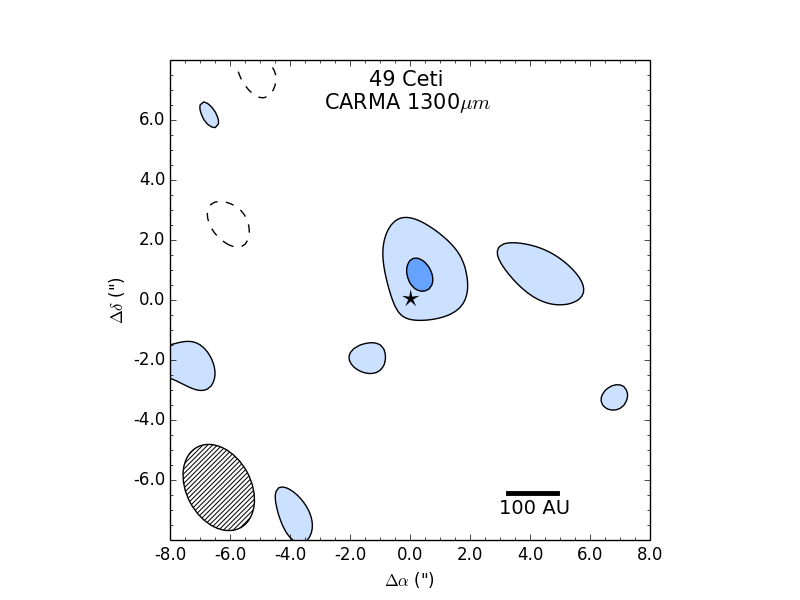
\includegraphics[width = 1\textwidth]{49CET_CARMA_16x16_1300um.png}
%\includegraphics{bonusBelt_200x600_KNAC_TriplePlot_highres.png}
\caption{1300$\mu$m CARMA image of the dust disk of 49 Ceti. The contours are [$-$2, 2, 4] $\times$ 520\,$\mu$Jy/beam (the RMS noise of the image). The beam size, represented by the shaded ellipse in the bottom left corner, corresponds to the resolution of the image, and is 3.04 $\times$ 2.17 arcsec. The position angle of the beam is 28.0$^{\circ}$. The scale bar of 100AU corresponds to 1.64 arcsec on the sky.} 
\label{fig:CARMA_image}
\end{figure}

%The optical depth of the disk can be estimated as the ratio of the infrared luminosity to the bolometric luminosity of the star. In 49 Ceti's case, photometric data from the literature suggest an optical depth of $10^{-3}$ for the dust, which is clearly optically thin. As such, we can

%The ratio of the infrared luminosity excess to the bolometric luminosity suggests 49 Ceti's dust disk is optically thin, and the double-peaked shape that is apparent in the SED (see figure SED) is consistent with a 

The structure of the disk is unresolved by CARMA, but we are still able to glean a reliable flux measurement by fitting a point source to the visibilities with the MIRIAD command \texttt{uvfit}. The derived flux is $2.1 \pm 0.7$\,mJy. If we fit with a Gaussian instead, we find that the major and minor axes are $1.6 \pm 1.8$ arcsec ($100 \pm 110$\,AU) and $0.3 \pm 1.7$ arcsec ($20 \pm 110$\,AU), respectively, indicating that the disk is unresolved along both the minor and major axis. 

\section{ALMA}
Figure \ref{fig:49CET_image} displays the image of 49 Ceti at 850\,$\mu m$. The image is also weighted using the Briggs weighting scheme, with robust = 0.5. In order to derive the integrated flux density, we fit a Gaussian to the visibilities at baselines $\leq$ 50 kilolambda, as these correspond to the largest angular scales in the data (see Figure \ref{fig:deprojected_DP_PL_Vis} for a plot of the deprojected visibilities). These baselines ``see" a disk that is well described by an elliptical Gaussian, and derive a flux of $17 \pm 3$\,mJy. Fitting a ring to all baselines severely underestimates the integrated flux, as any extended flux component would be missed by this model, but it does let us estimate where the peak emission is in the disk. The major axis of the ring is $3.822 \pm 0.003$ arcsec ($233.0 \pm 0.2$\,AU), and the minor axis is $0.626 \pm 0.003$ arcsec ($38.2 \pm 0.2$\,AU), implying that the structure is resolved along both the major and minor axes. The radius of this ring corresponds to the length of the semi-major axis and suggests that the brightest part of the disk is at roughly 117\,AU from the star. In addition, if we assume the disk is circular, we can derive the inclination. Denoting $a$ and $b$ the major and minor axes as seen by the observer and $i$ the inclination,

\begin{equation}
b = a \times sin (90 - i)
\end{equation}

The derived inclination is $80.6^{\circ} \pm 0.4^{\circ}$. The position angle ($PA$) is $-70.9^{\circ} \pm 0.4^{\circ}$. These values are consistent with those derived from subarcsecond Keck images of the inner disk by \cite{Wahh07}, who found $PA = -55^{\circ} \pm 10^{\circ}$ and $i = 60^{\circ} \pm 15^{\circ}$. They are also consistent with the values of $PA = -70^{\circ} \pm 10^{\circ}$ and $i = 90^{\circ} \pm 5^{\circ}$ derived from the outer gas disk observed with the Sub-Millimeter Array by \cite{Hugh08}.

If the 20$\%$ systematic uncertainty in calibrating the flux for radio instruments is taken into account, there is no statistical difference between the ALMA flux at 850$\,\mu m$ of $17 \pm 3$\,mJy and that from JCMT/SCUBA, also at 850$\,\mu m$, of $8.2 \pm 1.9$\,mJy \citep{Song04}. If we assume either a thermal spectrum ($F_{\lambda} \propto \lambda^{-2}$) or optically thin dust disk spectrum at long wavelengths ($F_{\lambda} \propto \lambda^{-3}$), we can compare the CARMA flux of $2.1 \pm 0.7$\,mJy at 1300$\,\mu m$ to the IRAM flux of $12.7 \pm 2.3$\,mJy derived at 1200$\,\mu m$ by \cite{Bock94}. With a thermal spectrum, we would expect the CARMA flux to be $10.8 \pm 2.0$\,mJy, but if the flux falls off as in an optically thin dust disk, it would be $10.0 \pm 1.8$\,mJy. Either way, there is a statistically significant difference between the IRAM flux and that derived from CARMA. As the error in the IRAM measurement is larger than the value we derived with CARMA, the value reported by \citeauthor{Bock94} is clearly spurious. %Because the values derived in this work are consistent with each other, we use these values later in 

\begin{figure}[ht]
\centering
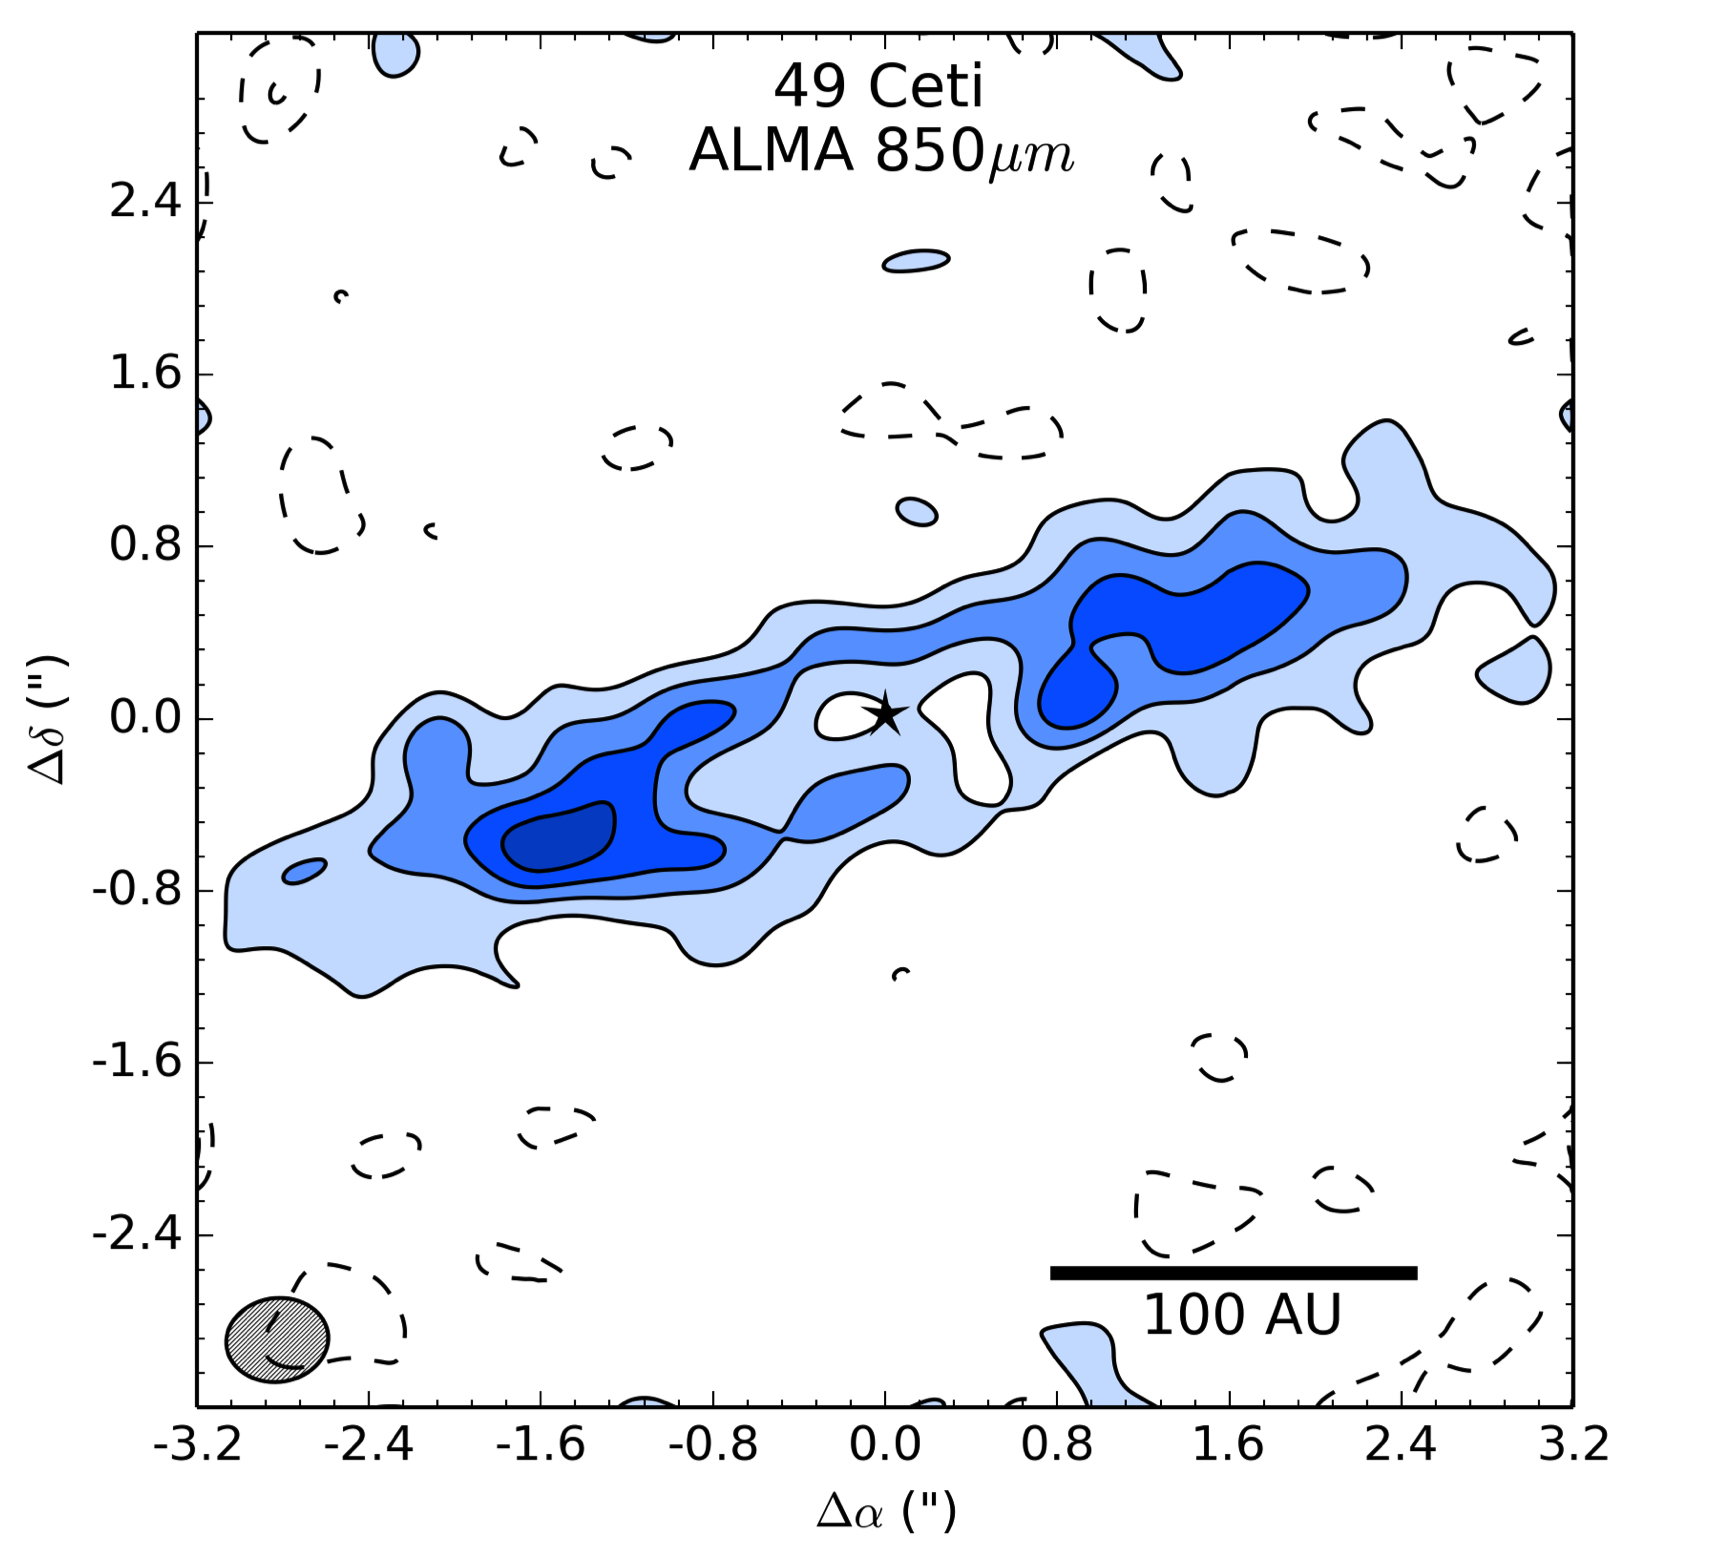
\includegraphics[width = 1\textwidth]{49CET_ALMA_square.png}
%\includegraphics{bonusBelt_200x600_KNAC_TriplePlot_highres.png}
\caption{850 $\mu$m ALMA image of the dust disk of 49 Ceti. The contours are [$-$2, 2, 4, 6, 8] $\times$ 58\,$\mu$Jy/beam (the RMS noise of the image). The beam size, represented by the shaded ellipse in the bottom left corner, is 0.47 $\times$ 0.39 arcsec. The position angle of the beam is -82.7$^{\circ}$. 2$\sigma$ emission extends 195AU from the star, and there seems to be an inner clearing. While the peak emission is slightly higher in the southeast than in the northwest of the disk, this difference is not statistically significant. The separation between the peaks is $\sim$ 3.3$''$ ($\sim$ 200\,AU) in the image and 3.8$''$ ($\sim$ 230\,AU) as derived by fitting a ring to the data with \texttt{uvfit}, suggesting that the density of the dust disk peaks between a radius of 100 and 115\,AU.} 
\label{fig:49CET_image}
\end{figure}




%\ifthenelse{\isodd{\thepage}}{\clearemptydoublepage}{}